\section{Background}
\subsection{Private cars as a mode of transport in urban settings}
\justify

%--talking points in this subsection
%Donald Shoup searching for parking
%city congestion
%private car mobility
%amount of cars in urban settings
%the space parked cars take

% parking policy:
%Goals of parking policy are numerous, for example optimal accessibility and traffic flow and maximising turn-over for shops (\cite{Marsden2006}).

% Shoup's High Cost of Free Parking -kirja, yritä etsii käsiin
The number of private cars is globally on the rise. According to one estimation, the world reached one billion cars in 2020 (\cite{Sperling2009}). International Organization of Motor Vehicle Manufacturers (OICA) estimates, that we were already at 950 million private cars in 2015 (\cite{OICA2020}). As the production of private cars is expected to continue, eyes must turn to managing the vast quantity of personal transportation in cities and in their surroundings. This is a question of mitigation of climate change, but also ensuring the economic performance of cities, and maximising the quality of life for urban citizens (\cite{Bertolini2003}).

Since the last century, urban landscapes have experienced change toward car based mobility, where streets have incrementally widened and parking standards continually increased. Much of the time this space has been taken from all other users of public space to accommodate cars (\cite{Cervero2017}). As cars have become a most common sight in cities, the mitigation of their adverse effects have become an important focus in policy. A major challenge cities face today is the relation of mobility of people and the urban land use. It has been shown that parking policy is an effective tool in the management of this challenge (\cite{Diallo2015}; \cite{Marsden2006}).

One goal of parking policy is an urban environment less dependant on private cars. However, a central issue in attempting to shape urban development in a direction that's less dependent on cars is that the alternatives fail to reach the quality of accessibility provided by private cars (\cite{Bertolini2003}). in \citeintext{Willson2013}, the author discusses that parking requirements have taken cities into a chokehold. They are responsible of creating the most wasteful sections of transport and land use complexes, the unoccupied parking spaces. To alleviate this situation, Willson has developed a 12-step toolkit to help planners make more informed decisions on the subject. These steps include points such as accounting for market conditions, and the consideration for alternative modes of transport, such as shuttle services or bicycles.

\newpage
\subsection{Accessibility}
\justify

Considering transportation of persons in cities, It may be thought that it is of highest priority to reach places as fast as possible. This is spatial mobility, movement which can be observed. However, people are ultimately not interested in measuring time units, but in social and economic interactions. It can then be said that the actual matter to focus in transporting persons in cities is not mobility, but accessibility. Accessibility can be defined as potential movement, observed through modeling. In accessibility, it is possible to attain a more realistic view into what is possible with available resources, such as time, and combine this matter with important issues regarding the sustainable development of cities. (\cite{Hodge1997}; \cite{Tenkanen2017}; \cite{Cervero2017})

First discussed by \citeauthor{Hansen1959} (\citeyear{Hansen1959}), accessibility as a concept has been widely studied in the decades that followed. In these first efforts Hansen succeeded in showing that locations in Washington D.C., United States, that had good accessibility were more likely to end up developed. These areas would also be developed at a higher density.

Torsten Hägerstrand's classic time geography approach developed further the idea that accessibility is a intricate complex of interdisciplinary tendencies. Individuals can be viewed as a bearers of action spaces of varying sizes and durations, which are determined by their social role, income, and how advanced technology they can access. Individuals are bound to their time budgets which are indivisible from certain constraints: the capacity, coupling, and institutional constraints (\cite{Wegener1999}; \cite{Hagerstrand1970}).

%Hodge asks how to navigate the intricate implications of accessibility, and reject the simplicity of distance or time as measure of accessibility (\cite{Hodge1997})
Continuing on Hägerstrand's action-space line of thinking, Zahavi (\citeyear{Zahavi1974}) proposed that individuals are not attempting to minimise travel time or cost required for a number of activities, but to maximise what is available to them considering their travel times and monetary budgets. Zahavi's theory can explain why the expansion of private car use has been as extensive as it has been. According to \citeintext{Wegener1999}, the theory sheds light why the motorisation in the twentieth century caused even longer and more car trips when travel speed gains were attained and why shopping centers in outskirts of cities can attract customers from ever more larger areas of influence.

More recently, \citeintext{Geurs2004} and \citeintext{Bertolini2003} have provided their definitions for accessibility. \citeauthor{Geurs2004} argues that accessibility should be associated with land use and transport systems in society and this would provide individuals with opportunities to take part in activities in different locations. According to \cite{Bertolini2003}, accessibility refers to the quantity and the diversity of spatial opportunities which can be reached within a certain amount of time.

\newpage
\subsection{Previous parking studies}
\justify
%Hyödynnä taustoittamisessa:
%\cite{Belloche2015}, On-street Parking Search Time Modelling and Validation with Survey-based Data
%\cite{Aryandoust2019}, City-scale car traffic and parking density maps from Uber Movement travel time data
%käytetty -- \cite{Axhausen1993}, Effectiveness of parking guidance and information systems: recent evidence from Nottingham and Frankfurt am Main
%\cite{Parmar2020}, Study on demand and characteristics of parking system in urban areas: A review

%parking search: adverse effects on traffic congestion (thompson 1998:ssa: parker 73, gillen 77, feeney 89)
Parking is an important part of a traffic system as all vehicles need a storage location when they are not in use. And due to increasing amount of cars, cities being built on private car mobility, and parking policy trying to find a balance between raising activity locally and not deterring visitors, motorists have been shown to spend a large percentage of their overall travel chain \textit{searching for parking} (\cite{Axhausen1991}; \cite{Marsden2006}; \cite{Shoup2006}). Searching for parking has been identified as a eminent source of urban congestion (\cite{Axhausen1993}), and parking policy improvements are much needed for most major cities (\cite{Benenson2008a}). According to \cite{Young1991}, the quantity and the location of parking affect:

\begin{itemize}
    \begin{singlespace}
        \item[--] the congestion on access roads and city streets
        \item[--] the efficiency and financial performance of public transport
        \item[--] comfort and safety levels of a city and the surroundings; and,
        \item[--] the form and functioning of the entire area as in its entirety
    \end{singlespace}
\end{itemize}

As such, parking policy is closely interlocked with potential conflict within different levels of government, city residents, holders of commercial interest, and other special interest groups (\cite{Ker1988}). It does not help matters that parking policy is an urgent matter in most major cities: \cite{Arnott2006} states that on-street parking may be utilised to over 100 percent capacity due to double parking, illegal curbside parking, and parking on the sidewalk. Inefficient parking policy also promotes \textit{cruising for parking}, a phenomenon which is partly a symptom of tension between demand and supply, and inefficiently low parking fees on-street (\cite{Shoup2004}; \citeyear{Shoup2006}). \citeintext{Martens2010} recognises three types of cruising for parking motorists: the commercial parkers, commuter parkers, and residential parkers.

Parking search problems originate from the mismatch between parking intentions of the motorists and available supply. In some more traditional cases, the mismatch can be addressed with expanding capacity or contstrain demand, but in other cases the problem is spatially and temporally specific, so that motorists' knowledge of local parking opportunities may be lacking, or road condition and layout is poor in specific places. (\cite{Axhausen1993})

%Motorists must base their choice on imperfect information, synthesise the initial perception with the additional information gained from previous as well as the current searching experiences (\cite{Thompson1998}).
Based on the works of \citeintext{Layzell1985} and \citeintext{Polak1989}, \citeauthor{Thompson1998} has defined the \textit{parking process} as a series of decisions by motorists based on updated knowledge gained from experience (\citeyear{Thompson1998}; figure~\ref{fig:parking-process-thompson}; a definition similar to this is also used by \cite{Guo2013}). The process commences on the start of searching for parking. Parking sites are examined and on the discovery of a favourable car park, a selection is made or the search continues (In \cite{Thompson1998} "car park" means both off-street parking garages as well as on-street parking that share common attributes). After leaving a selected car park, the next leg of the parking search process begins. \citeauthor{Thompson1998} state that motorists must make a choice on imperfect information, as aspects of the parking process are stochastic and opaque to individuals (\citeyear{Thompson1998}).

\begin{figure}[H]%
    \centering
    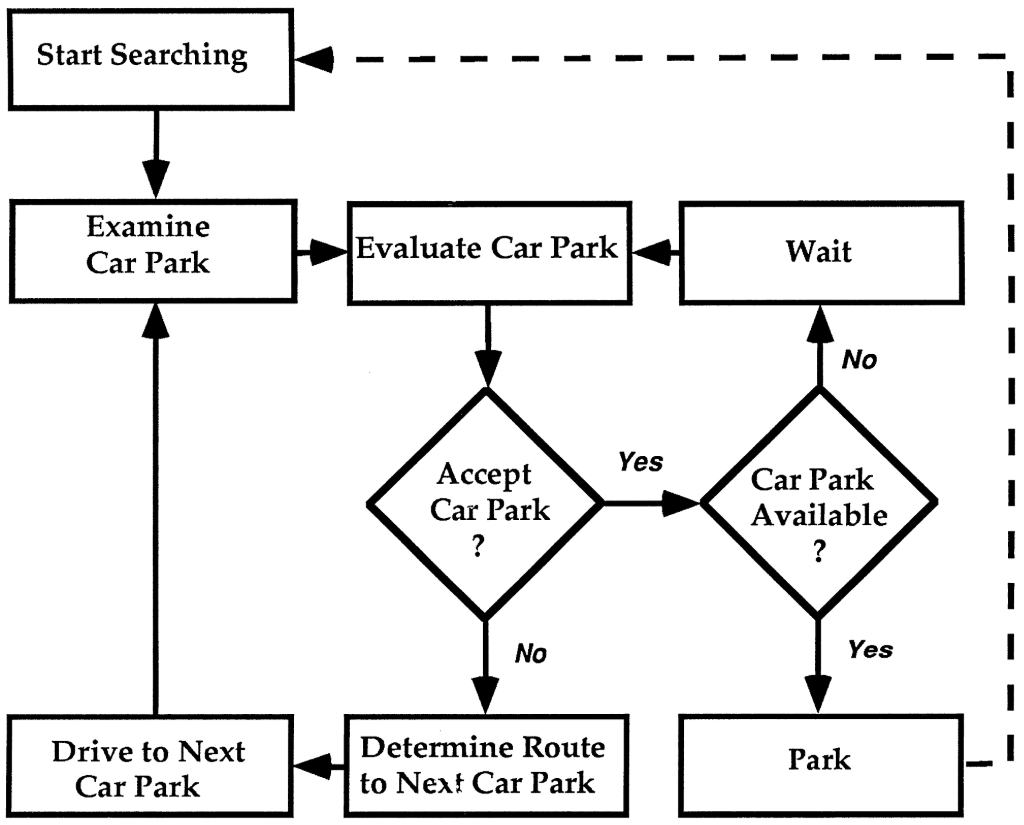
\includegraphics[width=.75\textwidth]{images/thesis_parking_search_process_thompson1998.PNG}
    \caption[Parking search process]{Defined by \citeauthor{Layzell1985} (\citeyear{Layzell1985}) and \citeauthor{Polak1989} (\citeyear{Polak1989}), parking choice may be considered as a search process in which motorists make linked decisions based on updated knowledge gained from experience. Parking choice Figure adapted from \citeauthor{Thompson1998} (\citeyear{Thompson1998}).}%
    \label{fig:parking-process-thompson}%
\end{figure}

% puhu tästä jossain? Broad estimations used in Helsinki Travel Time Matrix: item 0.42 min searching for parking, 2 min and 2.5 min walking in TTM18 (\cite{Tenkanen2020})
In \citeintext{Salonen2013}, the accessibility disparity is studied in a comprehensive manner. Many earlier accessibility studies are cast into doubt as they have been simplifying the subject matter, using methods that are not satisfactorily explained, or are simply incompatible. \citeauthor{Salonen2013} employ real data in finding compatible methods for calculating travel times for both private car and public transport. Introducing the \textit{door-to-door approach}, the researchers strove for maximum realism when calculating the duration of trips, or \textit{travel chains}. In the door-to-door approach for private car, all realistic parts of a journey is taken into account (figure~\ref{fig:door-to-door}). The trip starts at the point of origin (O), from where one walks to where their car is parked at (P). The car drive segment commences, and continues until the earliest place where one would like to park at. This is where the parking process starts (see figure~\ref{fig:parking-process-thompson}), and it continues until a parking place is found (O). Finally one walks to the final destination of their journey (D). The door-to-door approach for the private car draws attention to a severely understudied subject, the parking process at the end of every trip made. While they accurately demonstrated the events that take place in realistic private car trips, \citeauthor{Salonen2013} themselves touched the subject of parking process only fleetingly.

\begin{figure}[H]%
    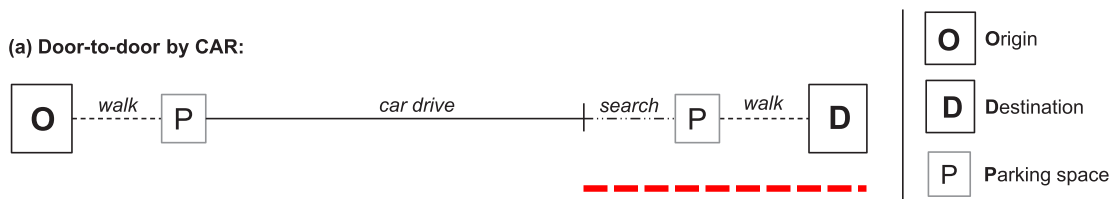
\includegraphics[width=\textwidth]{images/door2door.png}
    \caption[Door-to-door approach]{The entire travel chain of a private car using the door-to-door approach. The red dashed line represents the parking process segment of the travel chain. Figure adapted from \citeintext{Salonen2013}.}%
    \label{fig:door-to-door}%
\end{figure}

In this literary review to parking survey, it became apparent that most studies in this field employ a computational model to predict availability or use of parking spaces. Parking survey studies were sparse in number, and according to \citeauthor{Diallo2015} (\citeyear{Diallo2015}), this is because the cost or difficulty to access appropriate data. They also note that complexity and extent of such studies work as a detriment.

In one computational model, \citeintext{VanDerGoot1982}, based on a parking study in the city of Haarlem, the Netherlands, showed that walking time strongly influenced drivers' choice of parking. An additional finding was that with the parking purpose of "shopping", longer walking times led to longer parking times, and shorter walking times translated to shorter parking times. In addition, in shopping trips, destination choice is influenced by the parking search time (\cite{Axhausen1993}). In \cite{Thompson1998}, the authors found that long term experience in parking search does not automatically result in better choices. \cite{Guo2013} has explored parking search process through an agent-based model in which a supply and demand are incorporated with sequential game-theoric capacity model to account for motorists' psychological attitudes in university campuses in the United States. 

% kaikki Benenson et al. research, tutki
\citeintext{Benenson2008} proposes a parking process model that is spatially explicit and agent-based (termed "PARKAGENT"). This means that the model takes urban elements essential for investigating parking process into account and gives agents instructions on how to react in different circumstances, such as reactions to lack of parking spaces and parking enforcement efforts, to simulate parking behaviour of motorists. This paper shows that the addition of a new parking facility does not much improve average parking search time and walking distance for on-street parking motorists. This was because the new facility, essentially, would change the supply and demand scenario of that area, bringing in motorists to the area who have their journey destinations further away. The paper also states that traditional parking modeling is insufficient in saturated parking situations (most major cities), as it is not possible for these models to consider actions of independent agents which can make decision on exact GIS data. A detailed view into "PARKAGENT" is described in \citeintext{Martens2010} alongside with a performance comparison to a non-spatial model of parking. A finding from this paper states that if parking turnover is low for a location (15 percent in an hour), the parking occupancy level of 85 percent, proposed by \citeintext{Shoup2004}, can be raised up to 95 percent. Parking occupancy level can be adjusted with changes to parking fees. The paper also states that if parking turnover reaches 50 percent for an hour, the aforementioned optimisation does not work.

Furthermore, in \citeintext{Levy2015} propose the model termed "PARKFIT", an GIS algorithm for estimating parking patterns without the need for in-situ behavioural data, and an continuation for the research carried out on "PARKAGENT". If high-resolution infrastructure GIS layers are available, the algorithm can be used to produce estimations -- map views -- about average distances between private cars aiming for a specific destination and the actual destination, and additionally the proportion of cars that fail to find a parking spot. The model, however, does not include parking search time. 

% evaluate parking space availability at university campus \cite{Harris1997}
% on-street parking issues: \cite{Saltzman1997}
Simulation to evaluate parking space availability has also been utilised in, for example, \citeintext{Harris1997} and \citeintext{Saltzman1997}.

\newpage
\subsection{Parking time estimations}
\justify

In accessibility studies, the estimations and measurements for parking times are relatively scarce and a understudied subject. In Finland, a parking research project was made for the city of Tampere (\cite{Kalenoja2003}). The authors interviewed individuals that had just finished parking, and were enquired after circumstances behind the parking, such as the factors that made them decide on the current parking place and from what direction they drove to the parking place location. In this study, 55 percent of interviewees had parked into a parking garage, 33 percent on-street and 13 percent in other areas. Over 60 percent of all interviewees reported that a short walking distance to their destination was of importance. The average time to find a parking place was 0.42 minutes on weekdays (table~\ref{tab:kalenoja-parktimes}).

\begin{hyphenrules}{nohyphenation}
    \begin{table}[H]
        \centering
        \caption[Parking time results in Kalenoja \& Häyrynen 2003]{The average time (minutes) to find a parking place in different types of locations in Tampere, Finland (\cite{Kalenoja2003}).} 
        \label{tab:kalenoja-parktimes}
        \begin{tabular}{ llll }
            \toprule
            Parking place type  & Weekday   & Saturday  & Overall \\
            \midrule
            On-street           & 0.73      & 2.08      & 0.80 \\
            Other areas         & 0.16      & 0.38      & 0.18 \\
            Parking garages     & 0.22      & 0.55      & 0.33 \\
            Overall             & 0.42      & 0.65      & 0.46 \\
            \bottomrule
        \end{tabular}
    \end{table}
\end{hyphenrules}

Internationally, \citeintext{Shoup2006} has been a landmark paper in private car parking time research. Mustering all research there was available on \textit{cruising for parking}, Shoup was able to display a compilation of results from a wide temporal and spatial pool. The gathered data showed that a range of 8--74 percent of a total trip was spent in cruising for parking. The average time to find a curbside parking place was in the range of 3.5--14 minutes. Shoup himself acknowledges the wide variance, saying that in reality some cities may have zero time spent in cruising for parking, while in other locations most of a journey made with private car consists of it. Regarding time spent in searching for parking when traveling by private car, \citeintext{Polak1990} states that it may constitute up to 25 percent of the average total travel time. According to \citeintext{Axhausen1991}, motorists valuate short parking search times over the driving time, with parking search time being up to two times more valuable. 

\newpage
\subsection{Research in parcipatory GIS and map surveys}
\justify

%PPGIS bibliography and map survey considerations

%Do suburban residents prefer the fastest or low-carbon travel modes? Combining public participation GIS and multimodal travel time analysis for daily mobility research (\cite{Salonen2014}).
In \citeintext{Salonen2014}, participatory GIS (PPGIS) was employed in understanding what is the character of daily mobility in Helsinki Capital Region and how often fastest travel mode is selected in these trips. The data received from respondents was used in conjunction with advanced travel time models based on real world GIS data such as the Digiroad dataset by Finnish Transport Infrastructure Agency. In this study, respondents most often chose non-optimal travel modes on "bounded trips" (work, school, or day care) and that many of the respondents are ready to choose a slower, and less carbon emission intensive means of travel.

\citeintext{Laatikainen2015} made use of PPGIS in the context of accessibility to urban aquatic environments and the environmental justice perspective that is included in a premise such as this. Employing "SoftGIS" methodology, the researchers were able to gather large amounts of data from users of urban environments through a easy-to-use user interface on the internet (\cite{Kytta2011}). The researchers had the opportunity to make use Finnish Population Register to select group of potential respondents representative of the study area, the Helsinki Capital Region. In some of the results, researchers point out that even though water is almost omnipresent in Helsinki Capital Region, the utilisation of PPGIS revealed that proximity of a body of water does not have a clear influence on the real usage, or travel distances and times. This being said, the results showed that in many cases the body of water nearest to an individual was undesirable in some way, prompting the individuals to seek amenities along waterside further away. Also, while some areas of Helsinki Capital Region are closer to more water, this fact did not automatically mean good access because of matters such as land ownership issues.